\label{section:hardware}
\textit{This section describes the available hardware used in the project. Starting with the initial setup of the robot until the final setup on which the solution is implemented.}\\

This project makes use of a localization system based on ultrasonic transmitter-receiver pairs from GamesOnTrack (GoT). By default GoT localization works by having an ultrasonic receiver mounted on a moving vehicle and transmitter are mounted on the ceiling. The system to be used in this project is the newly developed reverse GoT system where the transmitter is mounted on the vehicle instead and the receivers on the ceiling. This should allow to increase the number of simultaneously tracked objects compared to the regular system (\textcolor{red}{TODO: max tracked for default GoT}).
Additionally, using the SLAM algorithm may provide ways to correct the systematic errors that the GoT system may exhibit in to non-line-of-sight situations.\\


\subsection{Range-finder - RPLidar}
A RPLidar unit is used for the purpose of obstacle avoidance. Through use of ROS RPLidar package a set of points is generated describing all visible obstacles around the robot. The position reported by GoT is expected to suffer from inaccuracies therefore a Kalman filter is to be developed for optimal position tracking.

\begin{figure}[H]
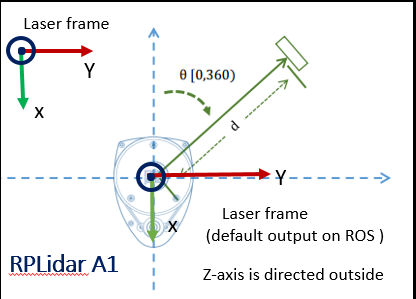
\includegraphics[scale=0.75]{Figures/rplidar_A1.png}
\centering
\end{figure}

\noindent In the first part of the project the Arduino board is replaced with a Raspberry Pi 3 board in favour of its increased processing power. Using a Raspberry Pi also allows using the Robot Operating System (ROS) and its SLAM implementations as well as adding vision based navigation methods. A RPLidar unit is used for the purpose of obstacle avoidance. Through use of ROS RPLidar package a set of points is generated describing all visible obstacles around the robot. The position reported by GoT is expected to suffer from inaccuracies therefore a Kalman filter is to be developed for optimal position tracking.\\

GoT transmitter/receiver\\
Teensy\\
Arduino Mega\\
RPLidar\\
Robot frame\\
DC motors\\
Future: Raspberry Pi\\